%!TEX root = ../main.tex
% APÉNDICE E — Diagramas UML
% Fuentes PlantUML en figuras/uml/*.puml. Para regenerar SVG y PDF:
%   java -jar plantuml.jar -tsvg -charset UTF-8 figuras/uml/0*.puml
%   (y convertir cada .svg a .pdf, por ejemplo con cairosvg o rsvg-convert)

\chapter{Diagramas UML}\label{apx:uml}

Este apéndice modela Tinku con los nueve diagramas UML pedidos. Todos se
construyeron a partir del código del repositorio
\texttt{smercadocarbone/usal-tinku}: las clases, estados, eventos, tiempos y
\emph{endpoints} que aparecen son los nombres reales del \emph{backend}
(Spring Boot), del \emph{frontend} (Next.js) y del servicio de
\emph{matching} (FastAPI). Las fuentes editables en PlantUML están en
\texttt{figuras/uml/}.

\section{Diagrama de actividad}

La Figura~\ref{fig:uml-actividad} recorre el ciclo completo de una clase,
desde la búsqueda hasta la calificación, con tres carriles: quien paga
(Estudiante adulto o Adulto Responsable), el \emph{backend} de Tinku y el
Tutor. Las decisiones siguen las reglas del sistema: la Solicitud de
Sesión cuando el beneficiario es menor, el tiempo límite de pago de
15 minutos, el modo \emph{bypass} de la pasarela, el no-show a los
10 minutos del inicio y el umbral del 50\,\% de duración efectiva que separa
una sesión finalizada de una interrumpida.

\begin{figure}[H]
    \centering
    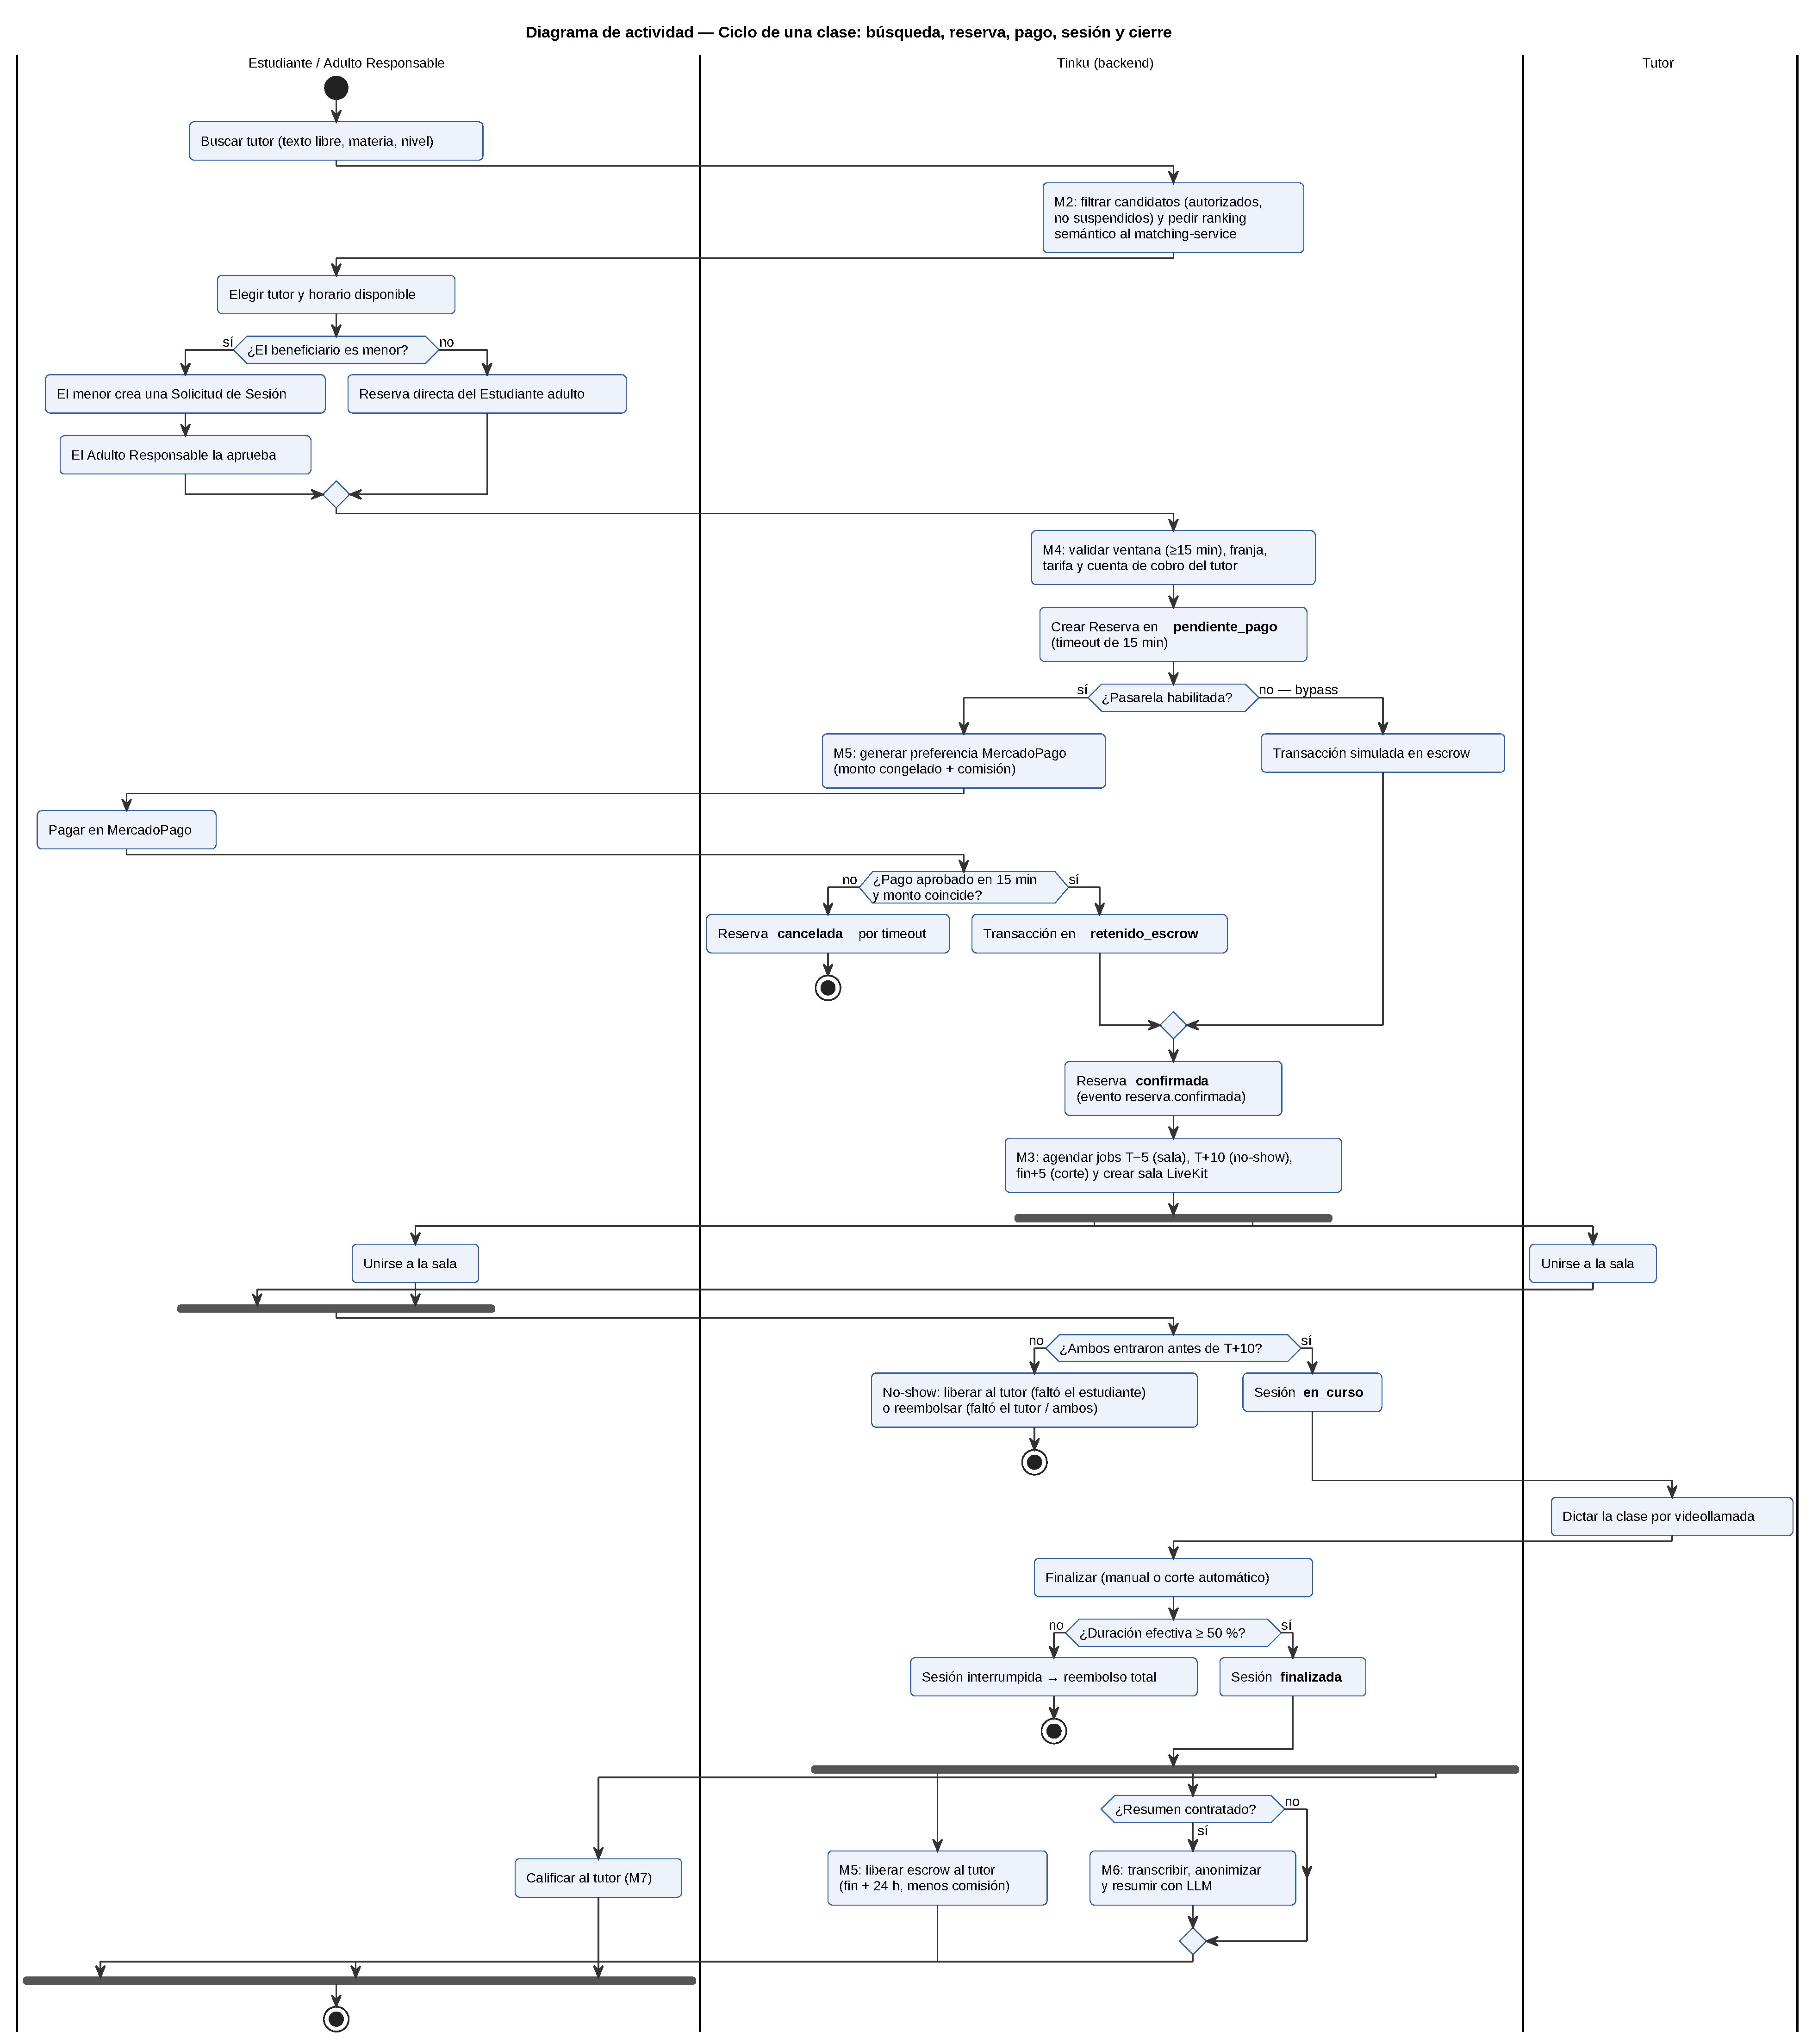
\includegraphics[width=\textwidth,height=0.8\textheight,keepaspectratio]{figuras/uml/01-actividad-reserva}
    \caption{Diagrama de actividad: ciclo de una clase}
    \label{fig:uml-actividad}
\end{figure}

\section{Diagrama de casos de uso}

La Figura~\ref{fig:uml-casos-uso} muestra los actores humanos (Visitante,
Estudiante adulto, Adulto Responsable, Estudiante menor, Tutor y
Administrador) y los sistemas externos (MercadoPago, LiveKit y el proveedor
del \gls{llm}). Estudiante adulto, Adulto Responsable, Estudiante menor y
Tutor especializan a Usuario registrado. Aprobar una solicitud incluye
reservar, reservar incluye pagar, y el kill-switch extiende la
participación en el aula.

\begin{figure}[H]
    \centering
    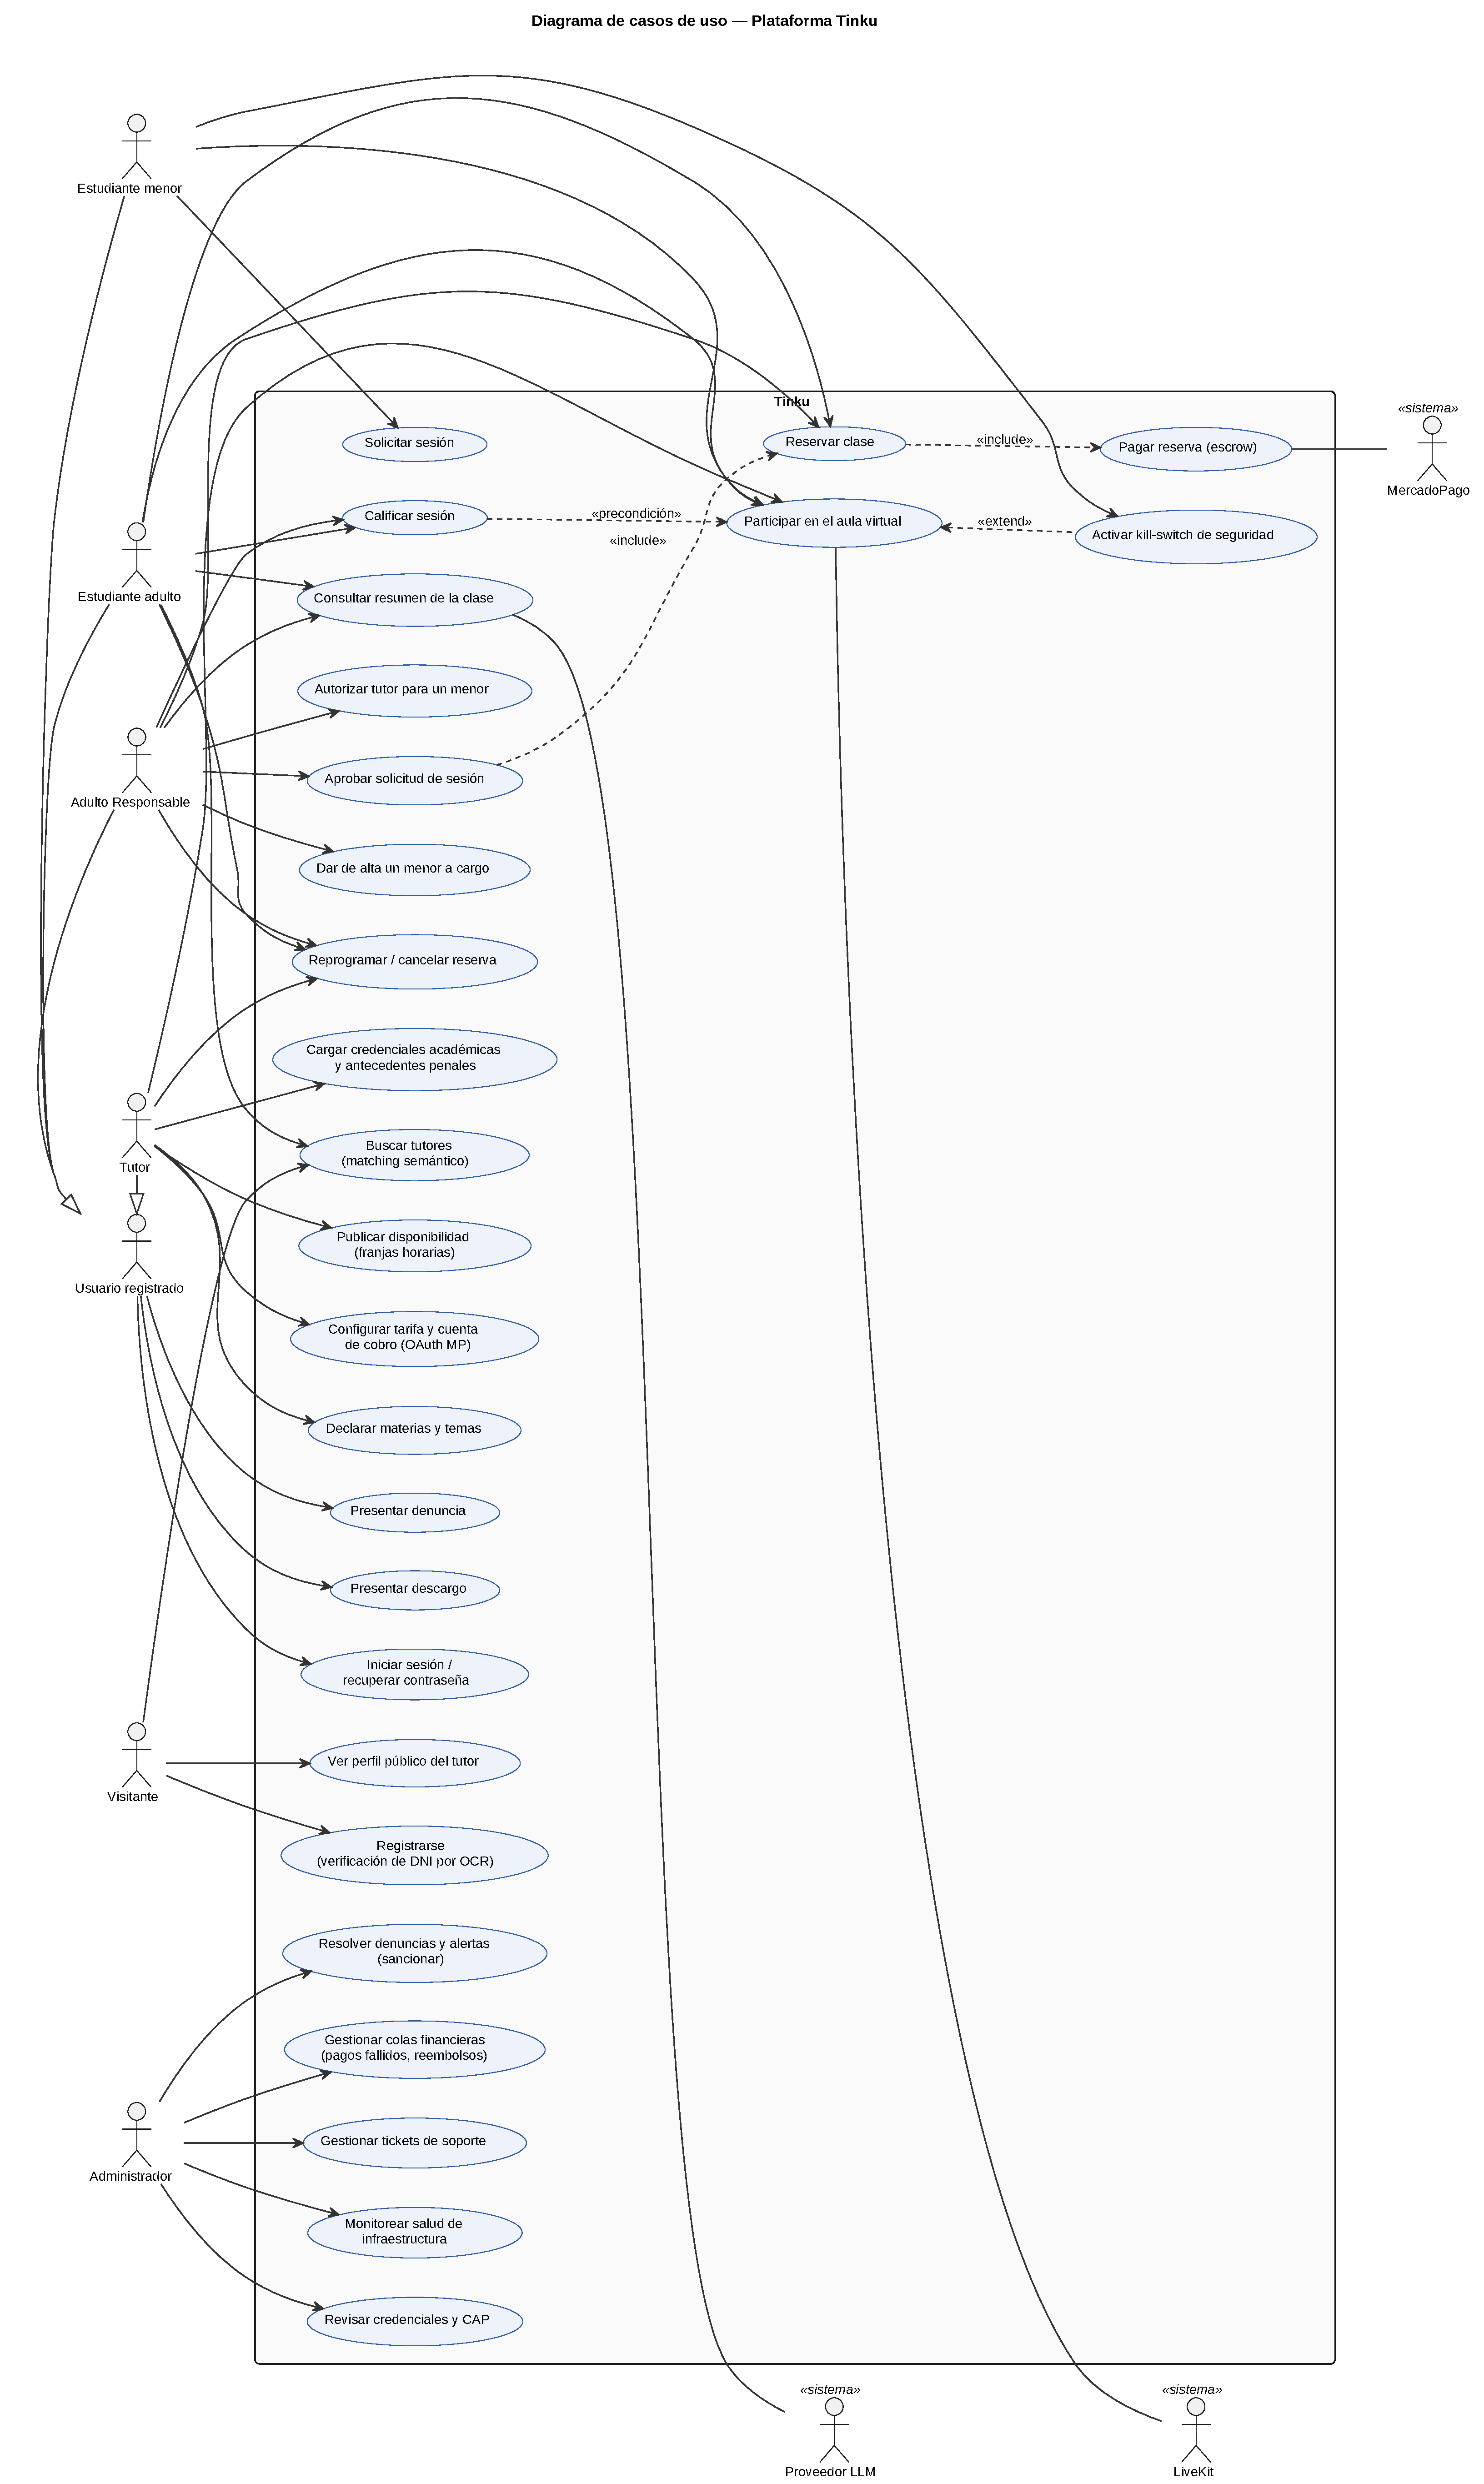
\includegraphics[width=\textwidth,height=0.8\textheight,keepaspectratio]{figuras/uml/02-casos-de-uso}
    \caption{Diagrama de casos de uso de Tinku}
    \label{fig:uml-casos-uso}
\end{figure}

\section{Diagramas de máquina de estados}

La Figura~\ref{fig:uml-estados-reserva} modela \texttt{EstadoReserva}. Una
Reserva nace en \texttt{pendiente\_pago} y pasa a \texttt{confirmada} cuando
se aprueba el pago. Termina en \texttt{finalizada}, \texttt{cancelada} o en
alguno de los tres estados de no-show. Mientras la clase transcurre, la
Reserva sigue en \texttt{confirmada}: el estado en vivo lo lleva la
Sesión de Aprendizaje. La Figura~\ref{fig:uml-estados-sesion} completa el
modelo con los estados de la \texttt{SesionAprendizaje} y de la
\texttt{Transaccion} en escrow, incluidas las pausas por denuncia y por
alerta de seguridad.

\begin{figure}[H]
    \centering
    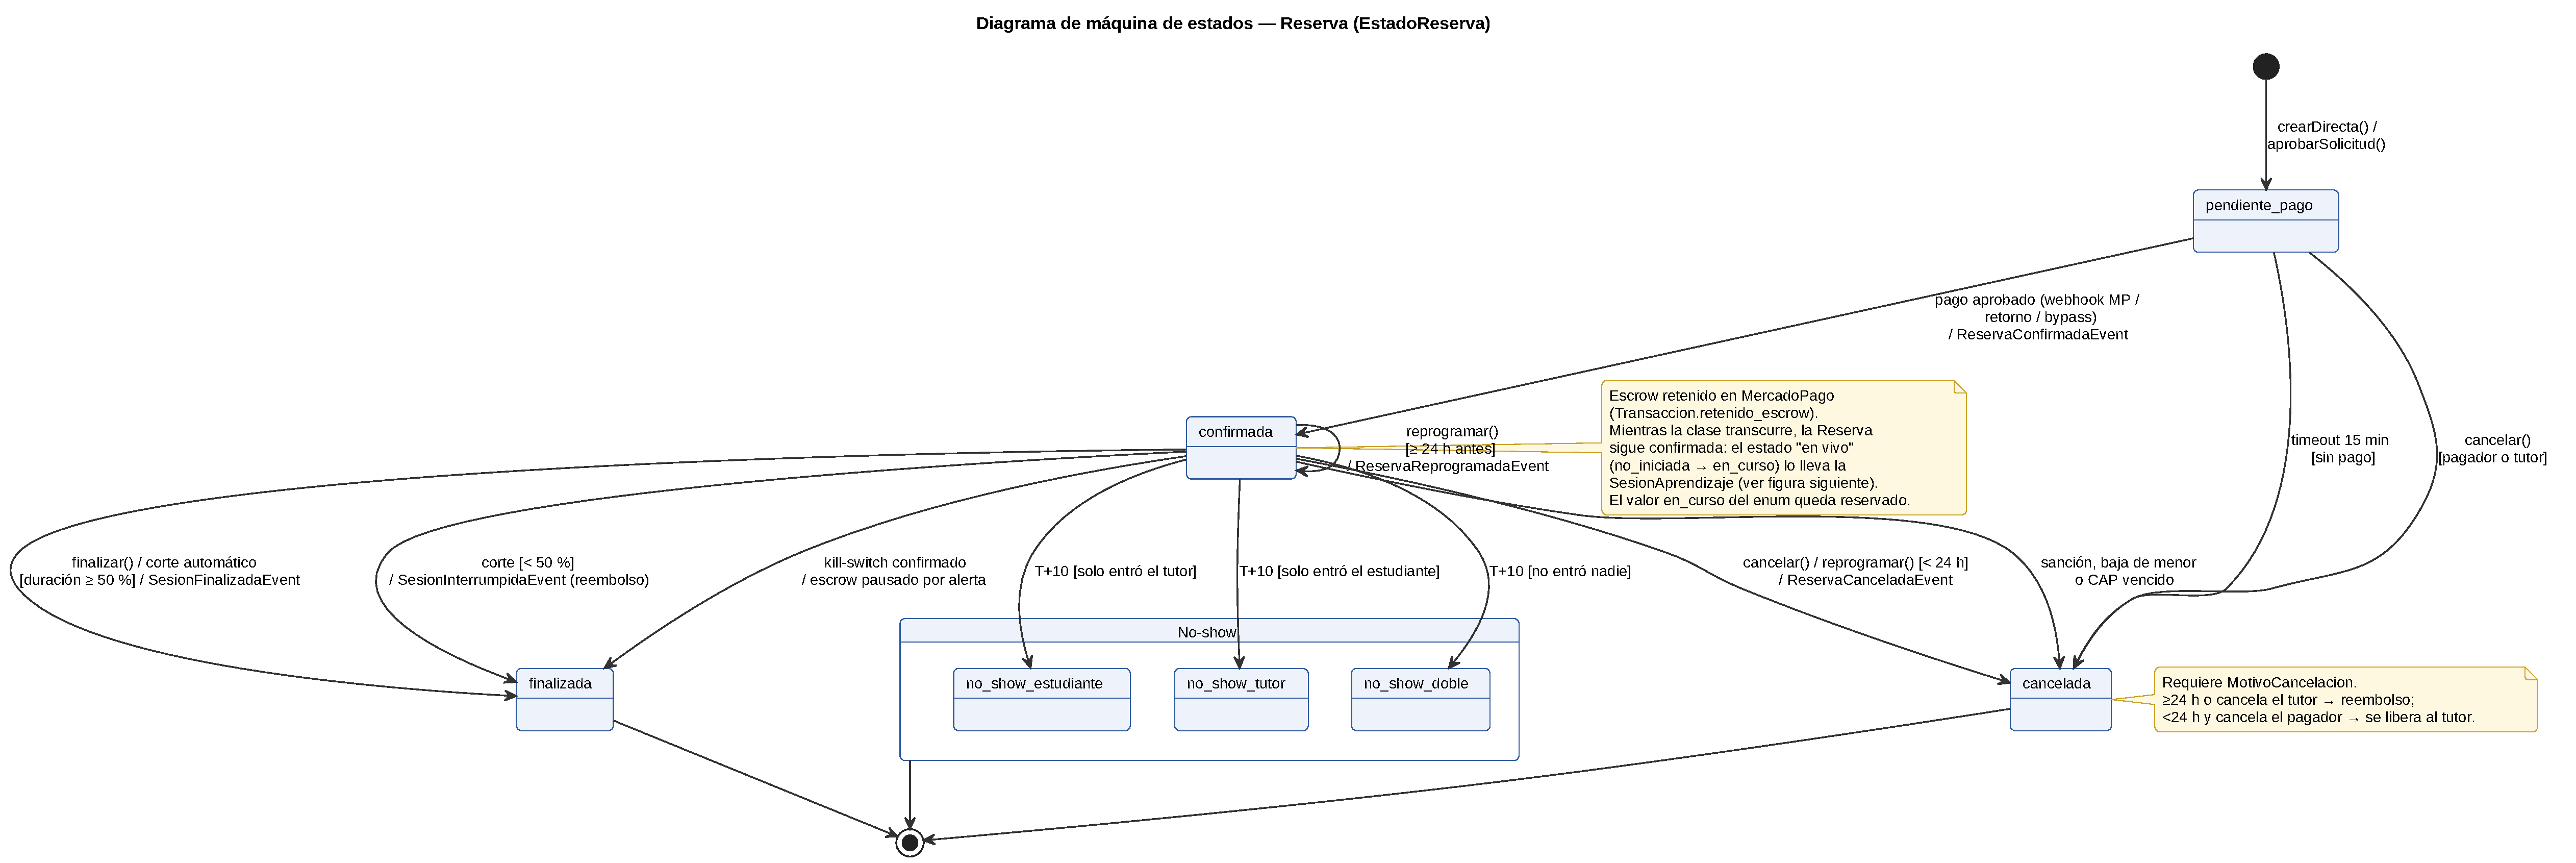
\includegraphics[width=\textwidth,height=0.8\textheight,keepaspectratio]{figuras/uml/03-maquina-estados-reserva}
    \caption{Diagrama de máquina de estados de la Reserva}
    \label{fig:uml-estados-reserva}
\end{figure}

\begin{figure}[H]
    \centering
    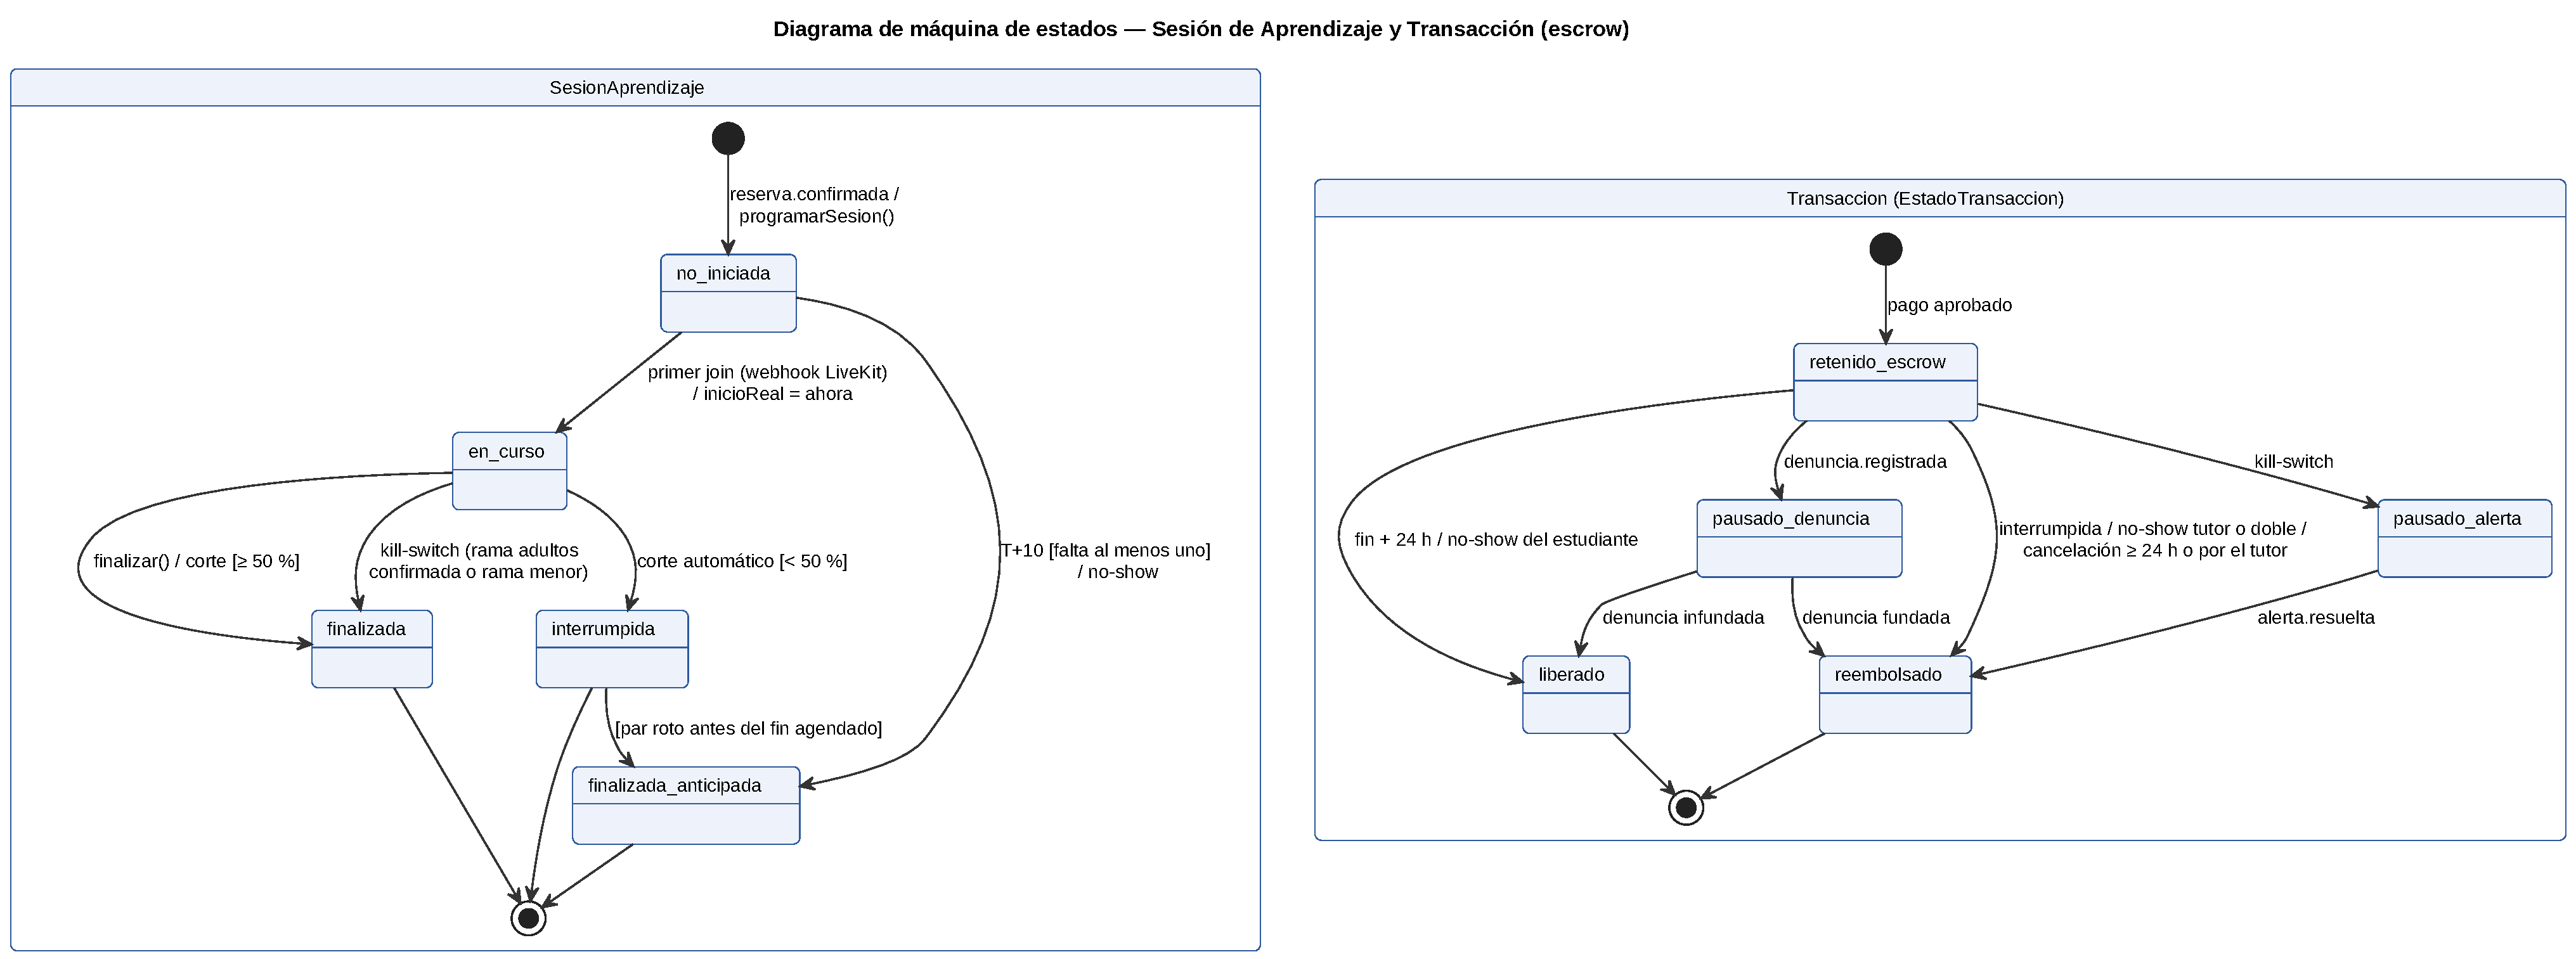
\includegraphics[width=\textwidth,height=0.8\textheight,keepaspectratio]{figuras/uml/03b-maquina-estados-sesion}
    \caption{Diagrama de máquina de estados de la Sesión de Aprendizaje y de la Transacción}
    \label{fig:uml-estados-sesion}
\end{figure}

\section{Diagrama de secuencia}

La Figura~\ref{fig:uml-secuencia} detalla la reserva directa y el pago con
escrow. El \emph{frontend} crea la Reserva y pide la preferencia de
MercadoPago. El \emph{webhook} firmado llega a \texttt{EscrowService}, que
vuelve a consultar el pago en MercadoPago, bloquea la fila de la Reserva y,
si el monto coincide con el precio congelado, crea la Transacción en
\texttt{retenido\_escrow} y confirma la Reserva. Esa confirmación publica
\texttt{ReservaConfirmadaEvent} para que el módulo de aula agende la
sesión.

\begin{figure}[H]
    \centering
    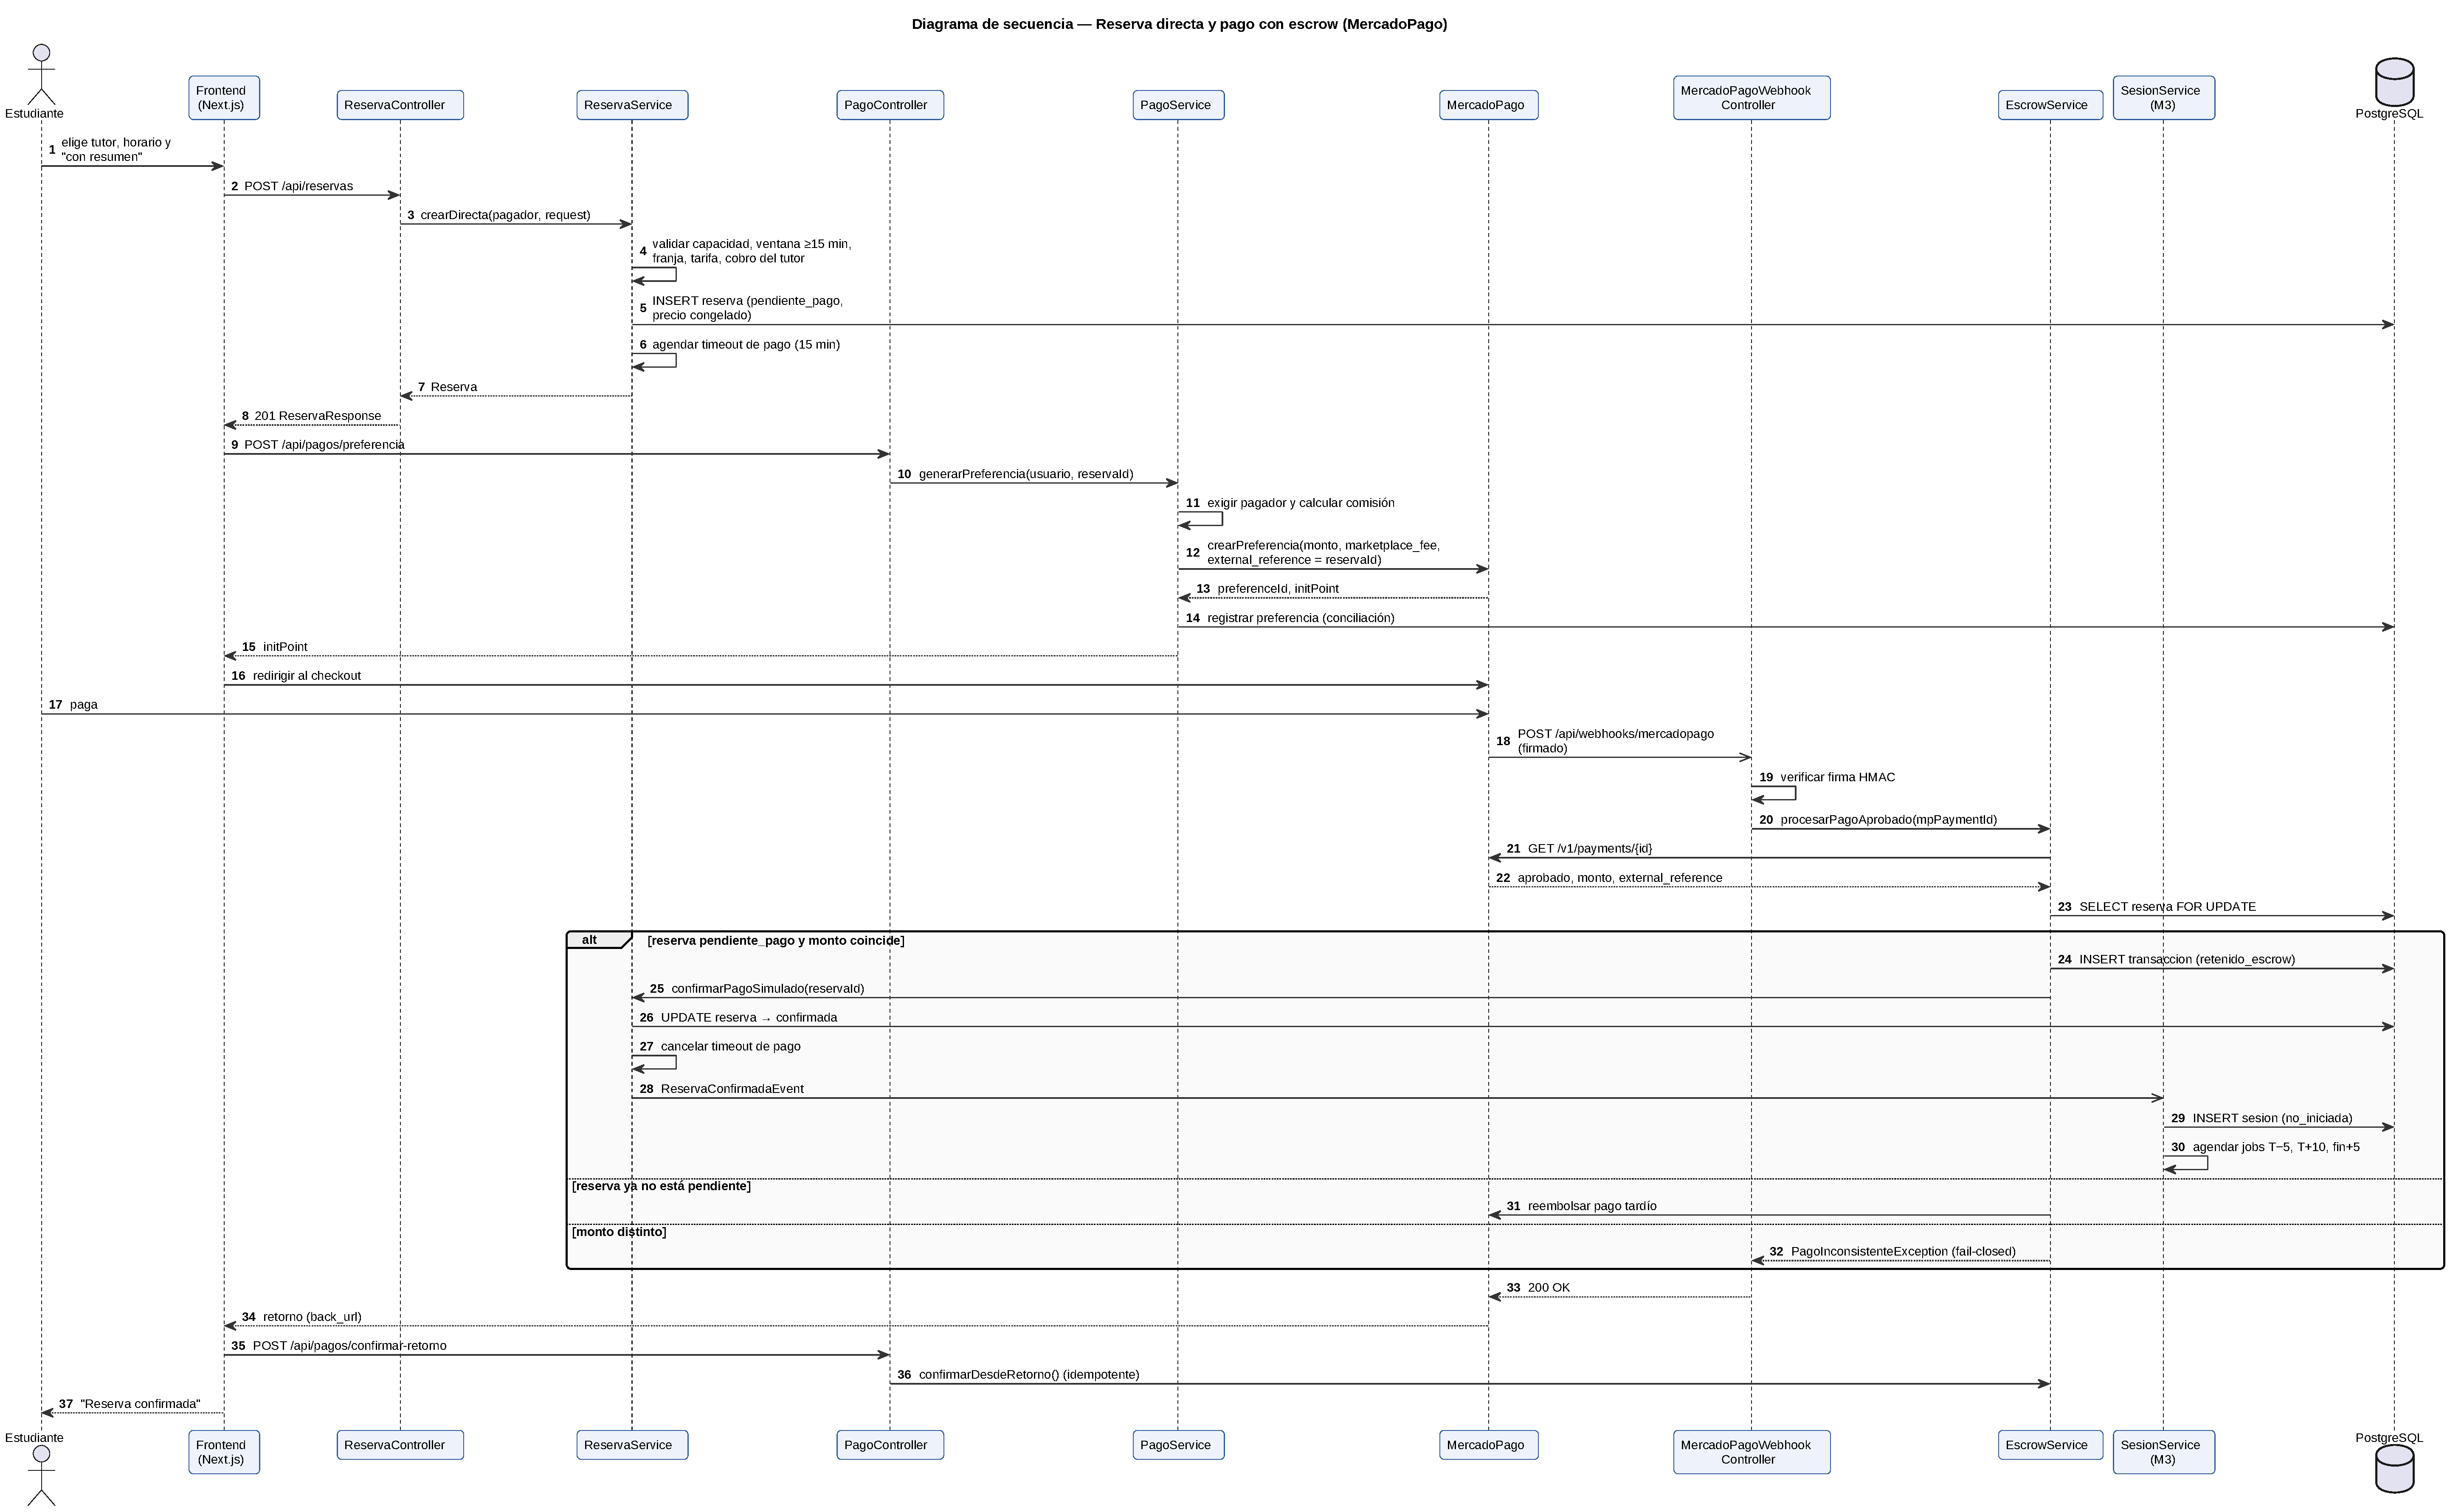
\includegraphics[width=\textwidth,height=0.8\textheight,keepaspectratio]{figuras/uml/04-secuencia-reserva-pago}
    \caption{Diagrama de secuencia: reserva y pago con escrow}
    \label{fig:uml-secuencia}
\end{figure}

\section{Diagrama de comunicación}

La Figura~\ref{fig:uml-comunicacion} muestra, con mensajes numerados, los
objetos que colaboran para entrar al aula virtual y cerrar la clase: la
emisión del token de LiveKit, los \emph{webhooks} de ingreso y salida, la
cancelación del job de no-show, el corte automático y los eventos que
reciben los módulos de pagos y de resumen.

\begin{figure}[H]
    \centering
    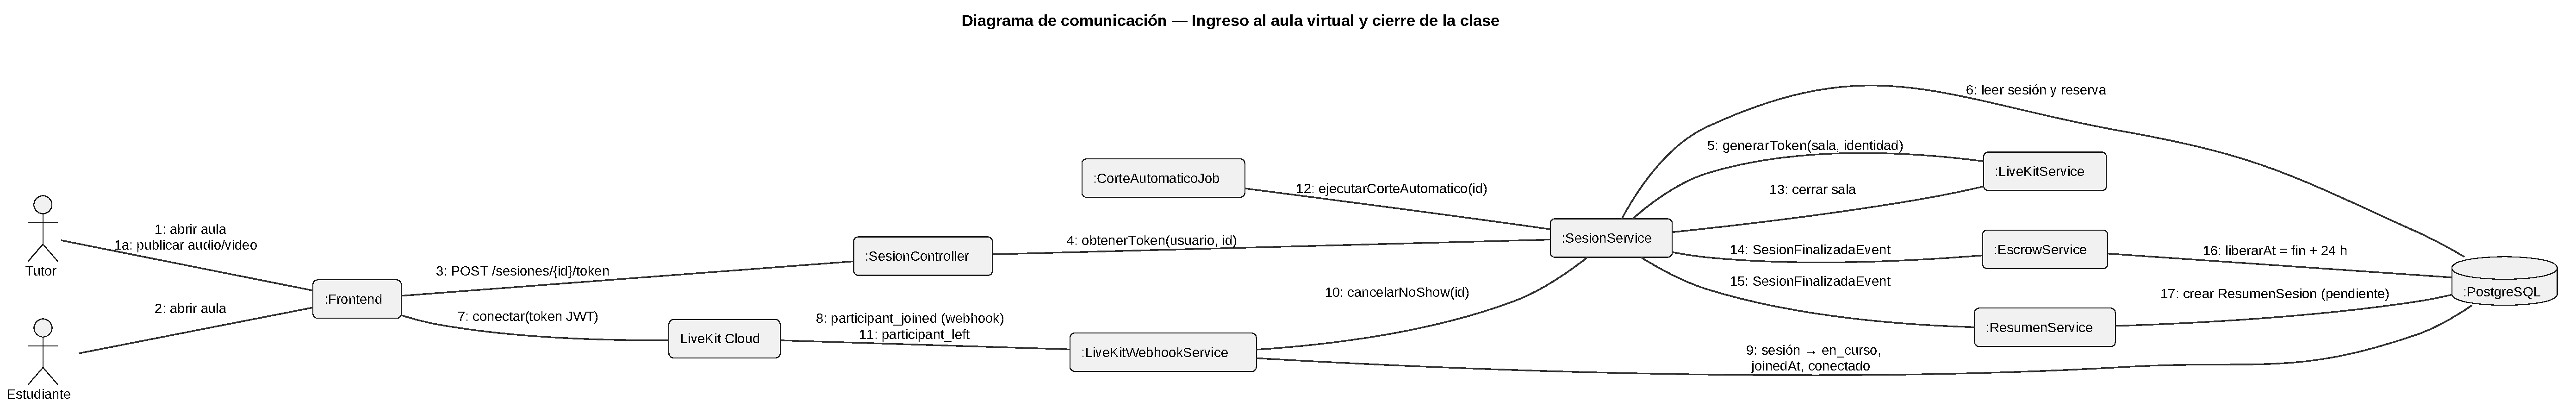
\includegraphics[width=\textwidth,height=0.8\textheight,keepaspectratio]{figuras/uml/05-comunicacion-aula}
    \caption{Diagrama de comunicación: aula virtual}
    \label{fig:uml-comunicacion}
\end{figure}

\section{Diagrama de tiempos}

La Figura~\ref{fig:uml-tiempos} ubica en una línea de tiempo los plazos de
una clase de 60 minutos: pago dentro de los 15 minutos, creación de la sala
en T$-$5, decisión de no-show en T$+$10 y corte automático 5 minutos
después del fin agendado. En ese momento se fija \texttt{liberarAt}, y el
pago se libera al Tutor 24 horas después del fin.

\begin{figure}[H]
    \centering
    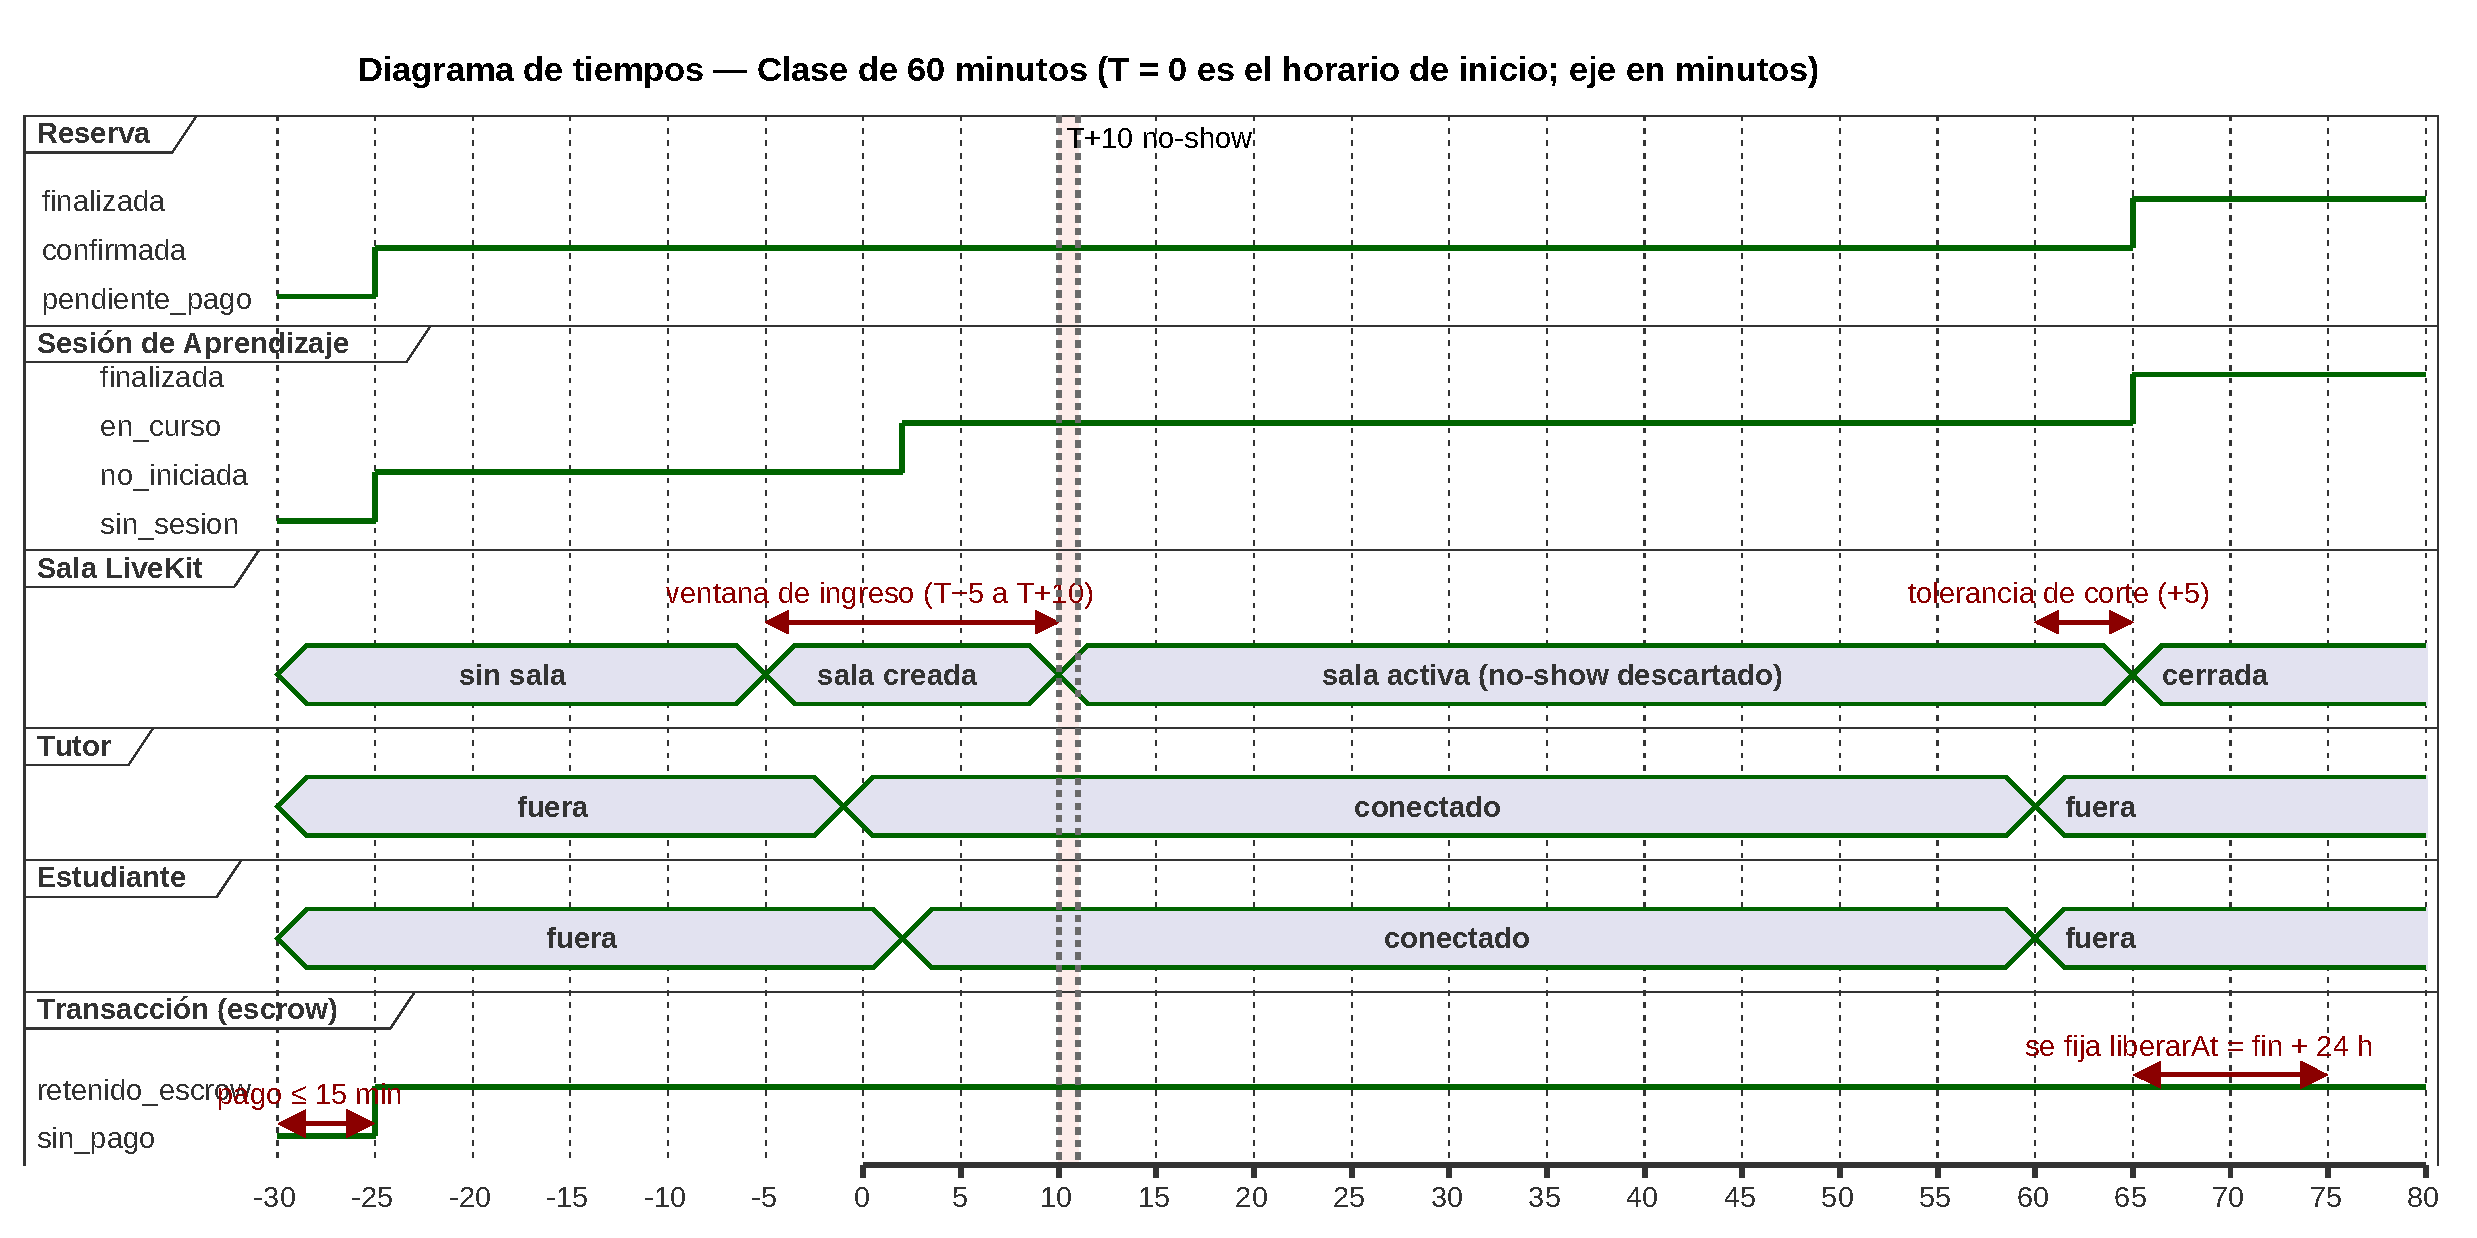
\includegraphics[width=\textwidth,height=0.8\textheight,keepaspectratio]{figuras/uml/06-tiempos-sesion}
    \caption{Diagrama de tiempos de una sesión}
    \label{fig:uml-tiempos}
\end{figure}

\section{Diagrama de visión general de interacciones}

La Figura~\ref{fig:uml-vision-general} encadena las interacciones del
sistema como fragmentos \texttt{ref}: búsqueda, solicitud o reserva
directa, pago, ingreso al aula, no-show o kill-switch, cierre y, en
paralelo, liberación del escrow, resumen automático y calificación.

\begin{figure}[H]
    \centering
    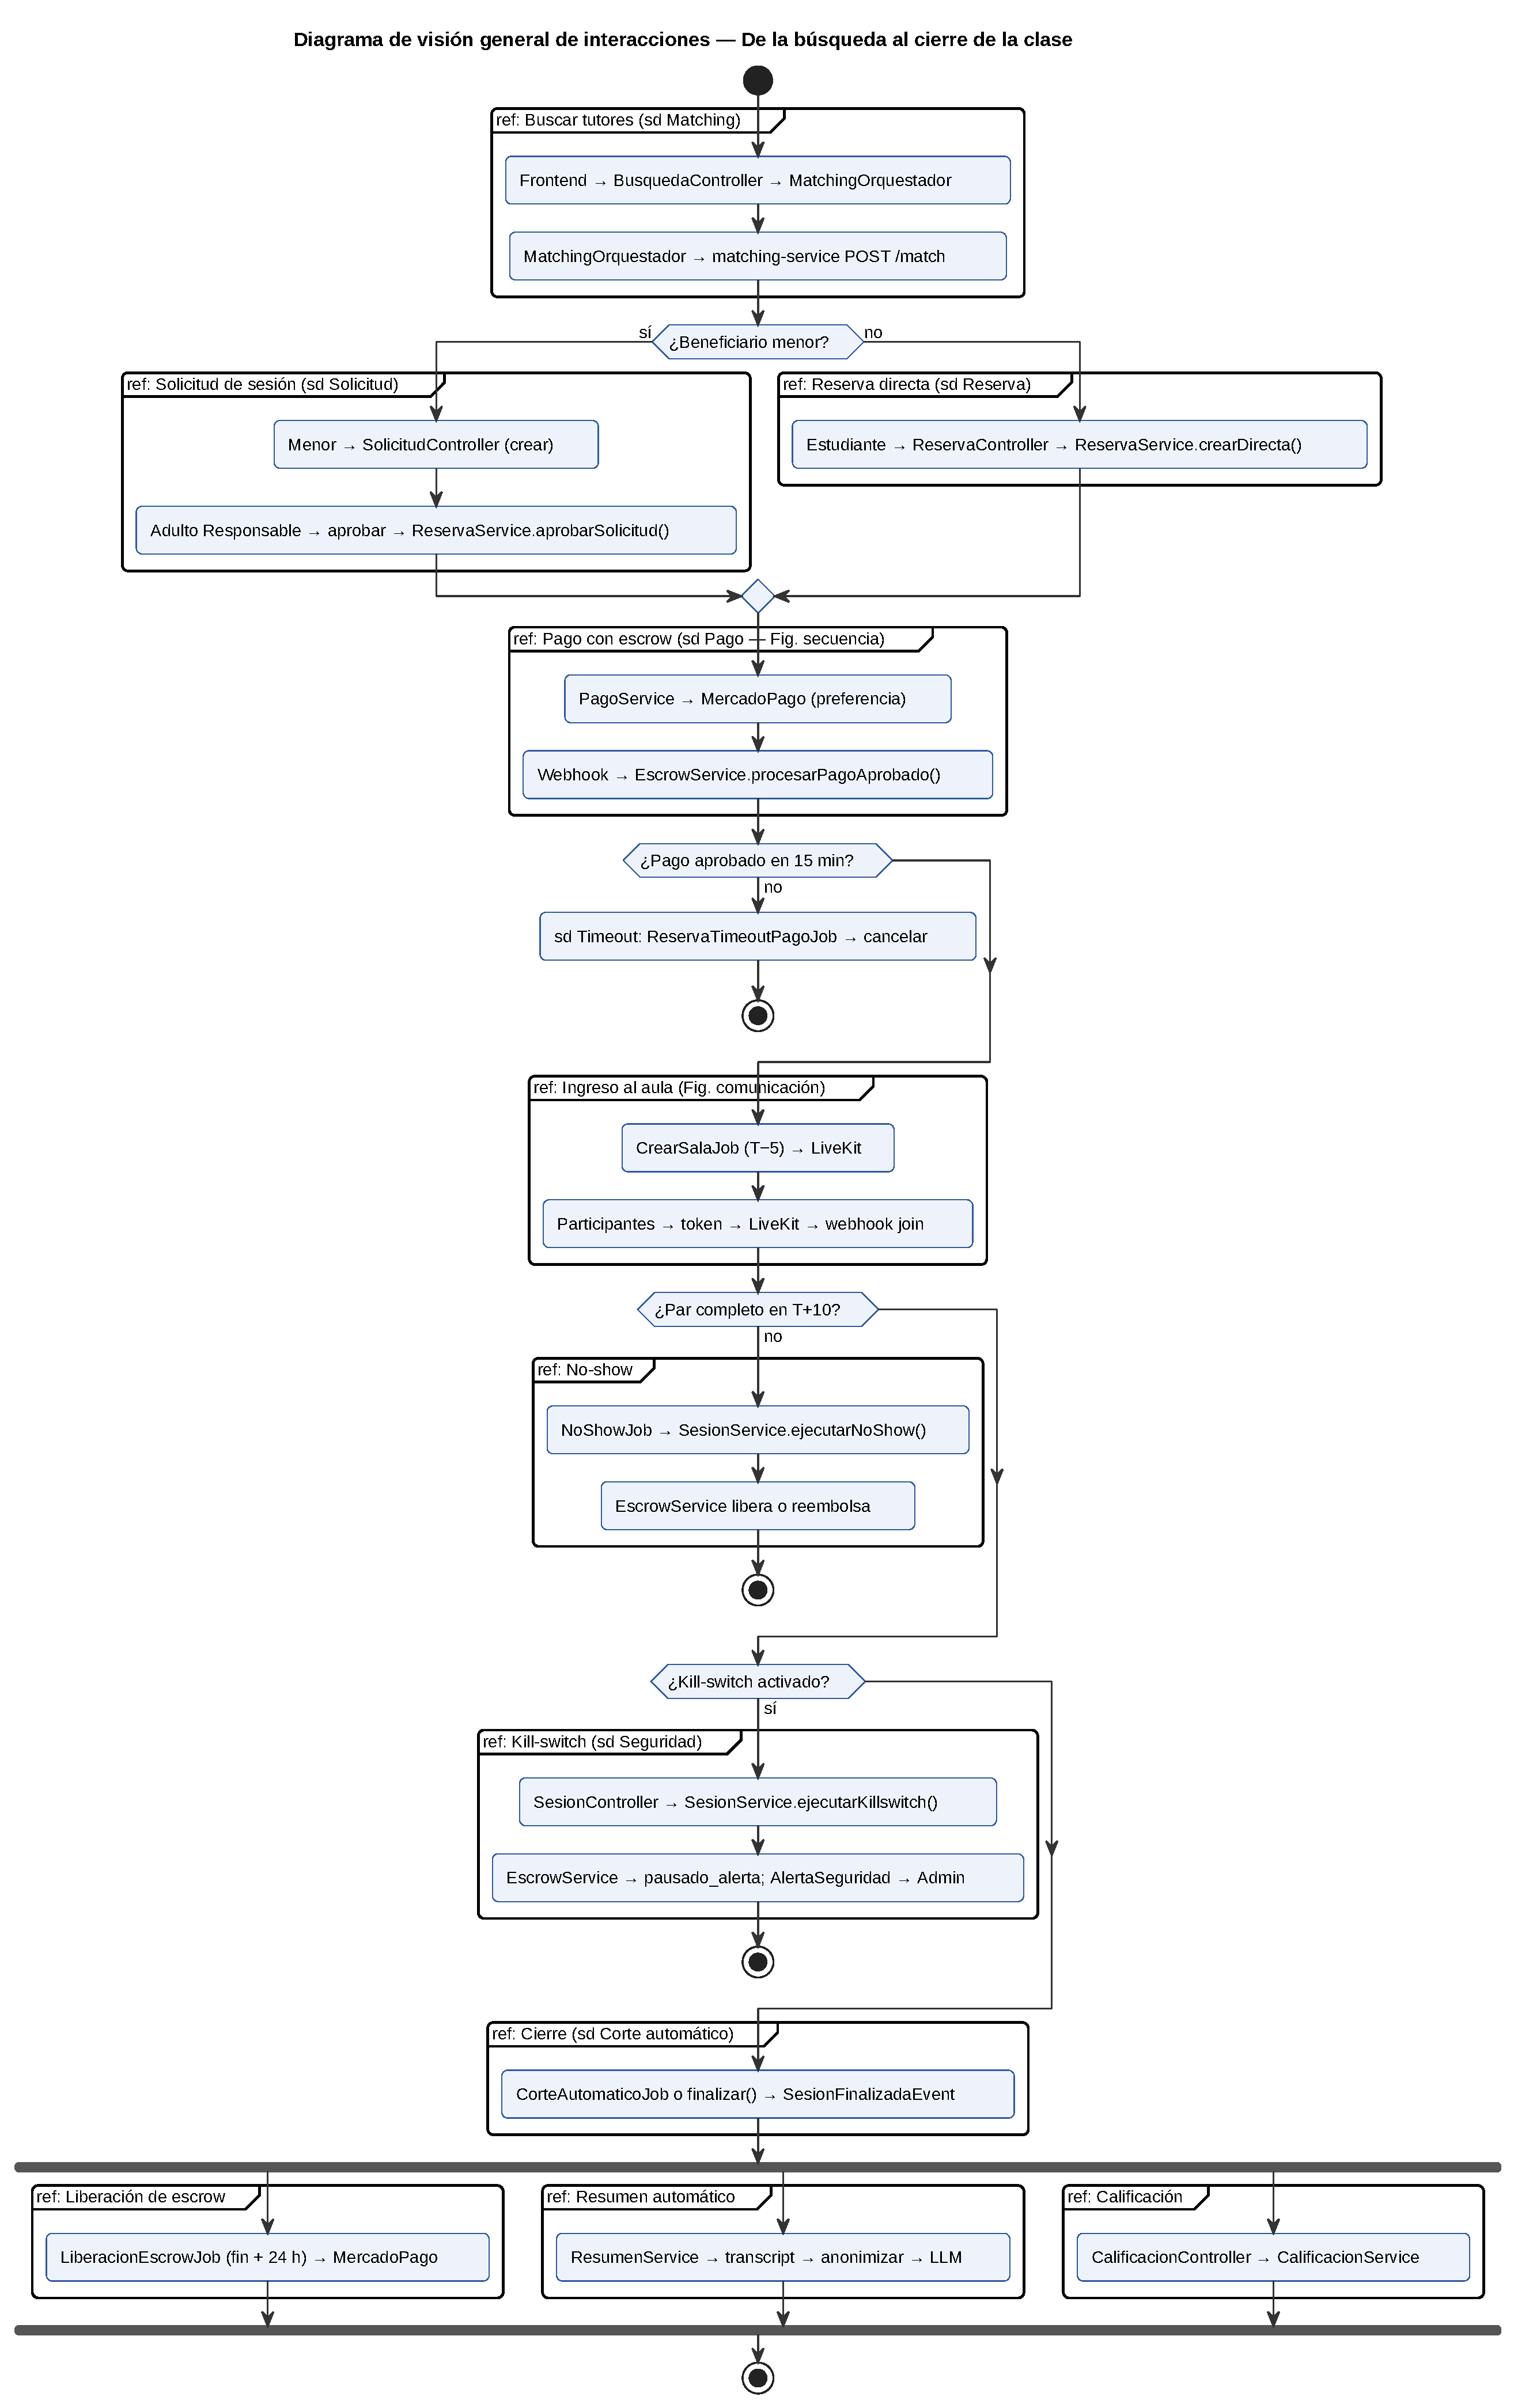
\includegraphics[width=\textwidth,height=0.8\textheight,keepaspectratio]{figuras/uml/07-vision-interacciones}
    \caption{Diagrama de visión general de interacciones}
    \label{fig:uml-vision-general}
\end{figure}

\section{Diagrama de clases}

La Figura~\ref{fig:uml-clases} presenta las entidades del dominio agrupadas
por módulo (M1 a M9), con sus atributos principales, sus enumeraciones de
estado y sus multiplicidades. \texttt{Usuario} concentra las identidades:
una Reserva lo referencia tres veces (pagador, beneficiario y tutor), y un
menor se vincula con su Adulto Responsable por una autorreferencia.

\begin{figure}[H]
    \centering
    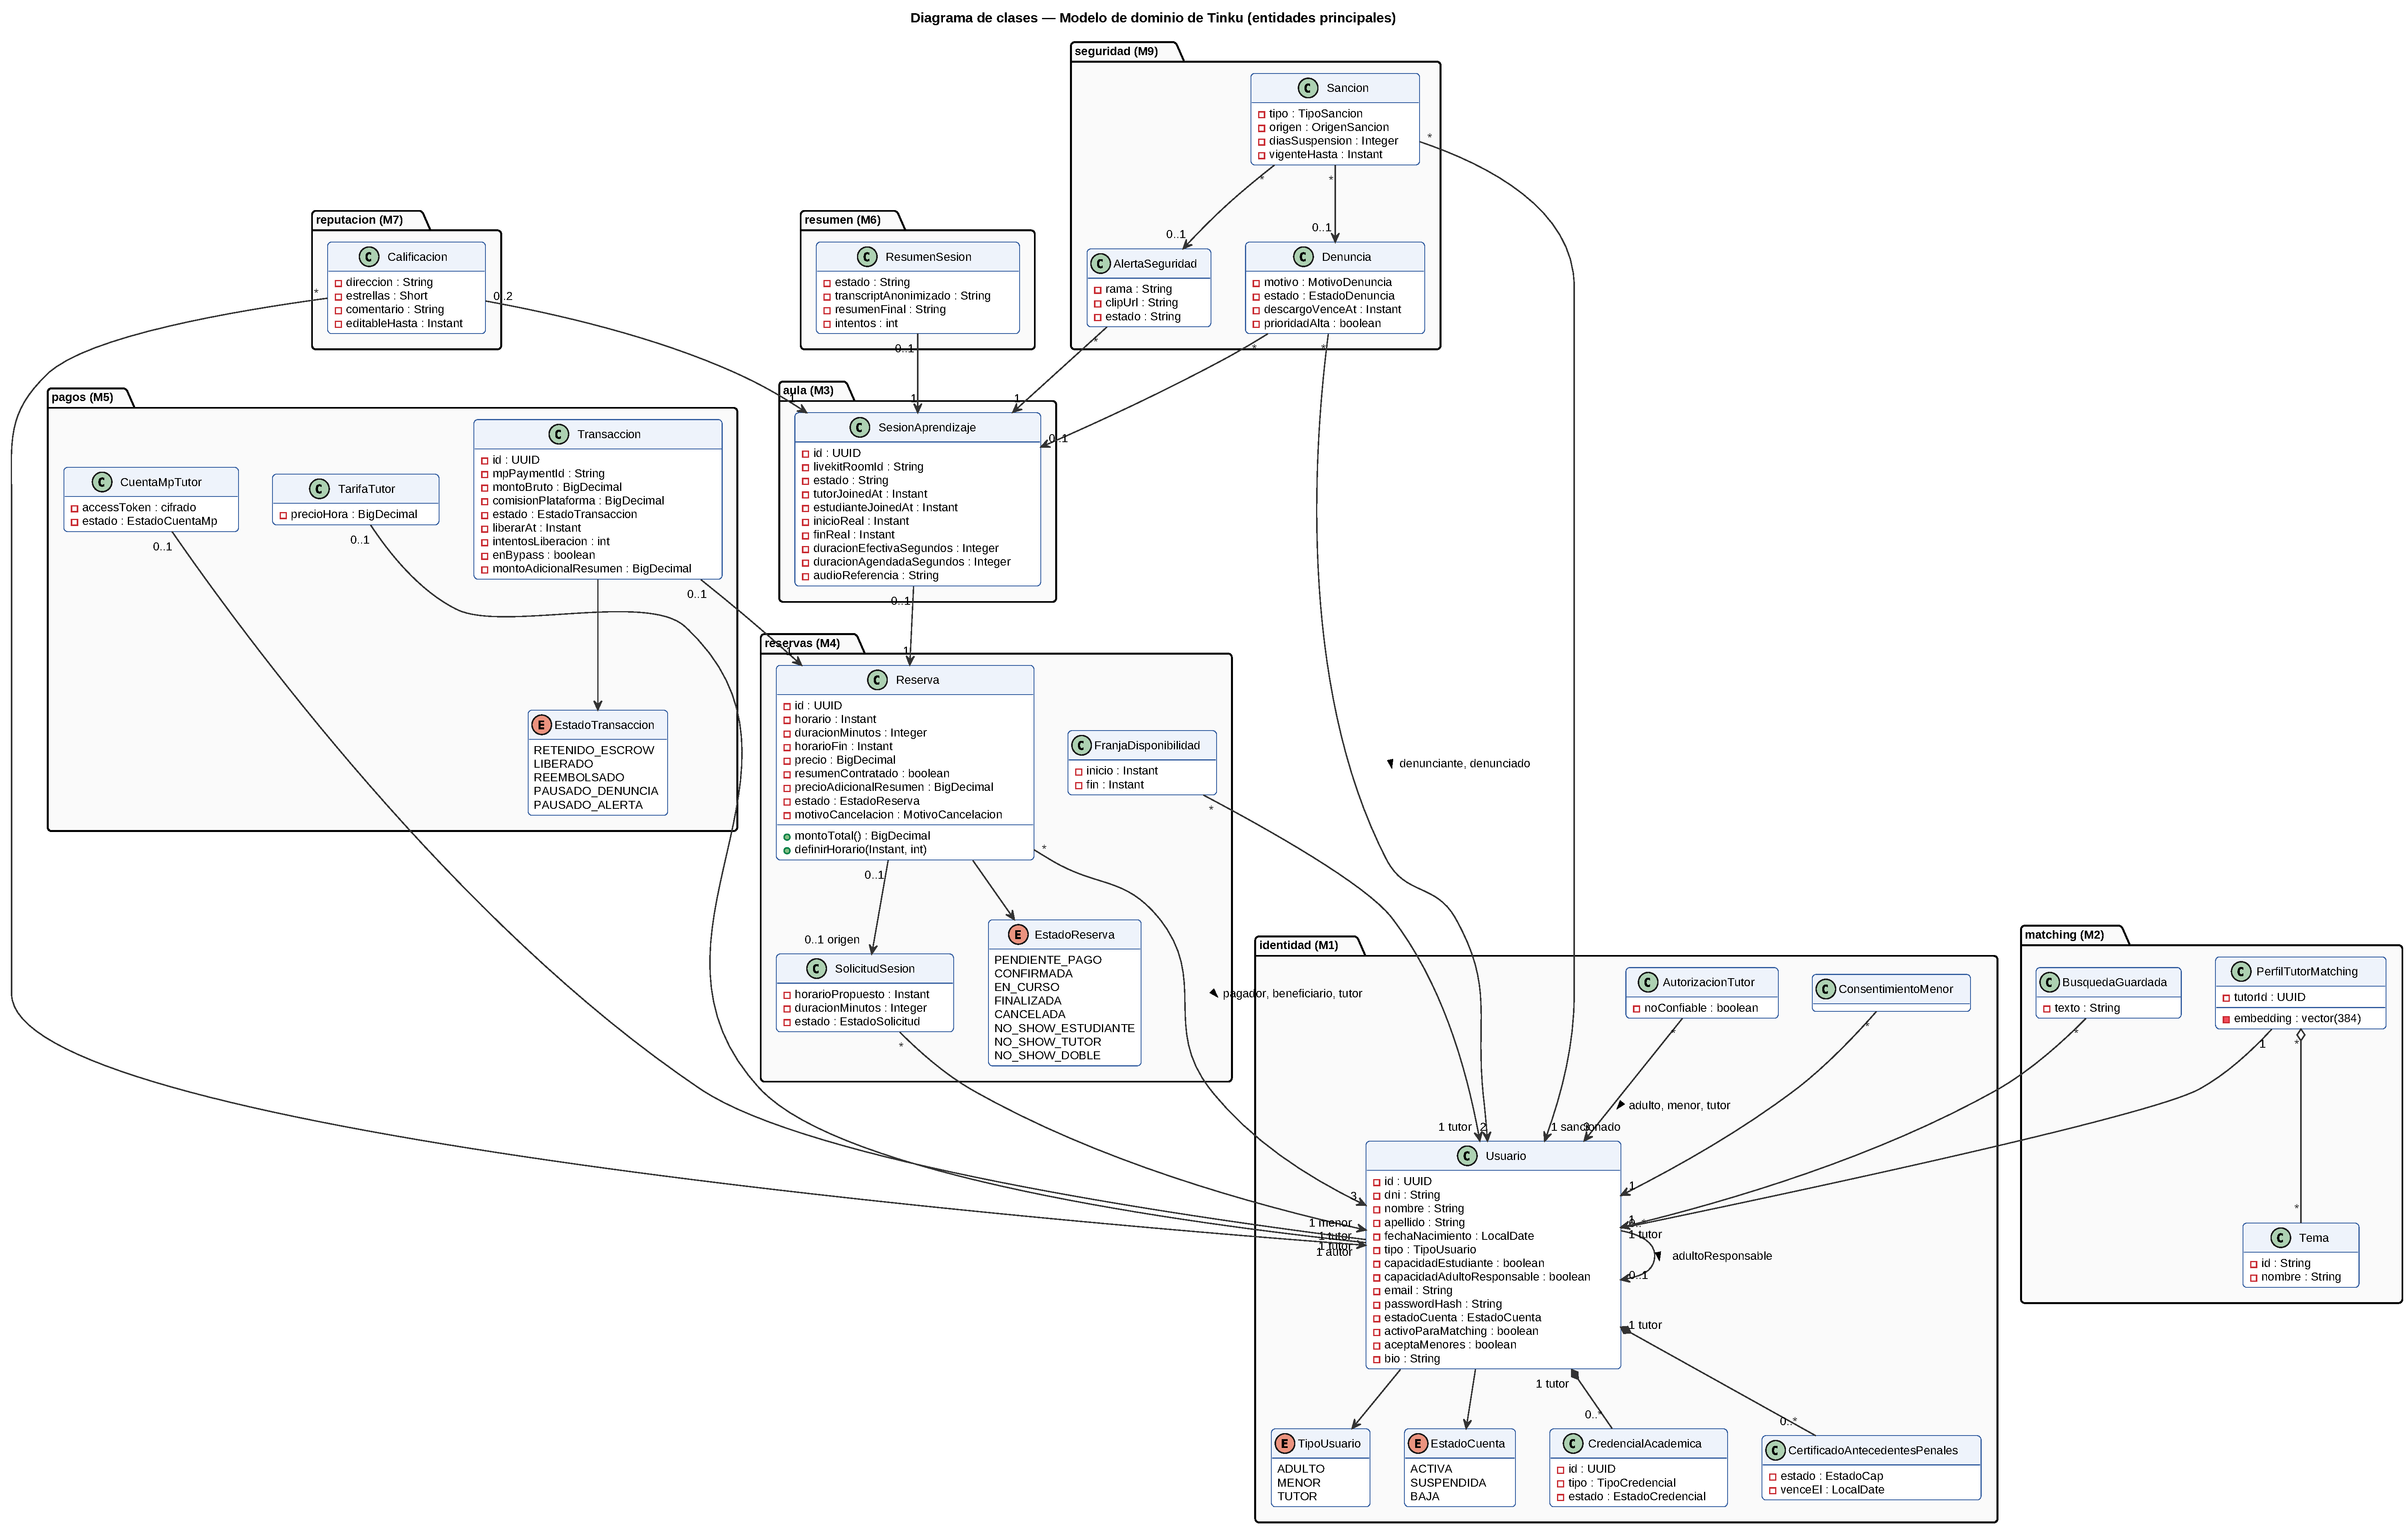
\includegraphics[width=\textwidth,height=0.8\textheight,keepaspectratio]{figuras/uml/08-clases}
    \caption{Diagrama de clases del modelo de dominio}
    \label{fig:uml-clases}
\end{figure}

\section{Diagrama de componentes}

La Figura~\ref{fig:uml-componentes} muestra el despliegue lógico: el
monolito modular Spring Boot con sus nueve módulos y el planificador
Quartz, el \emph{frontend} Next.js, el servicio de \emph{matching} en
Python (el único proceso separado), PostgreSQL con pgvector, el
\emph{backup} cifrado y los servicios externos. Las flechas punteadas entre
módulos son eventos de aplicación. El único ingreso desde internet es el
túnel de Cloudflare.

\begin{figure}[H]
    \centering
    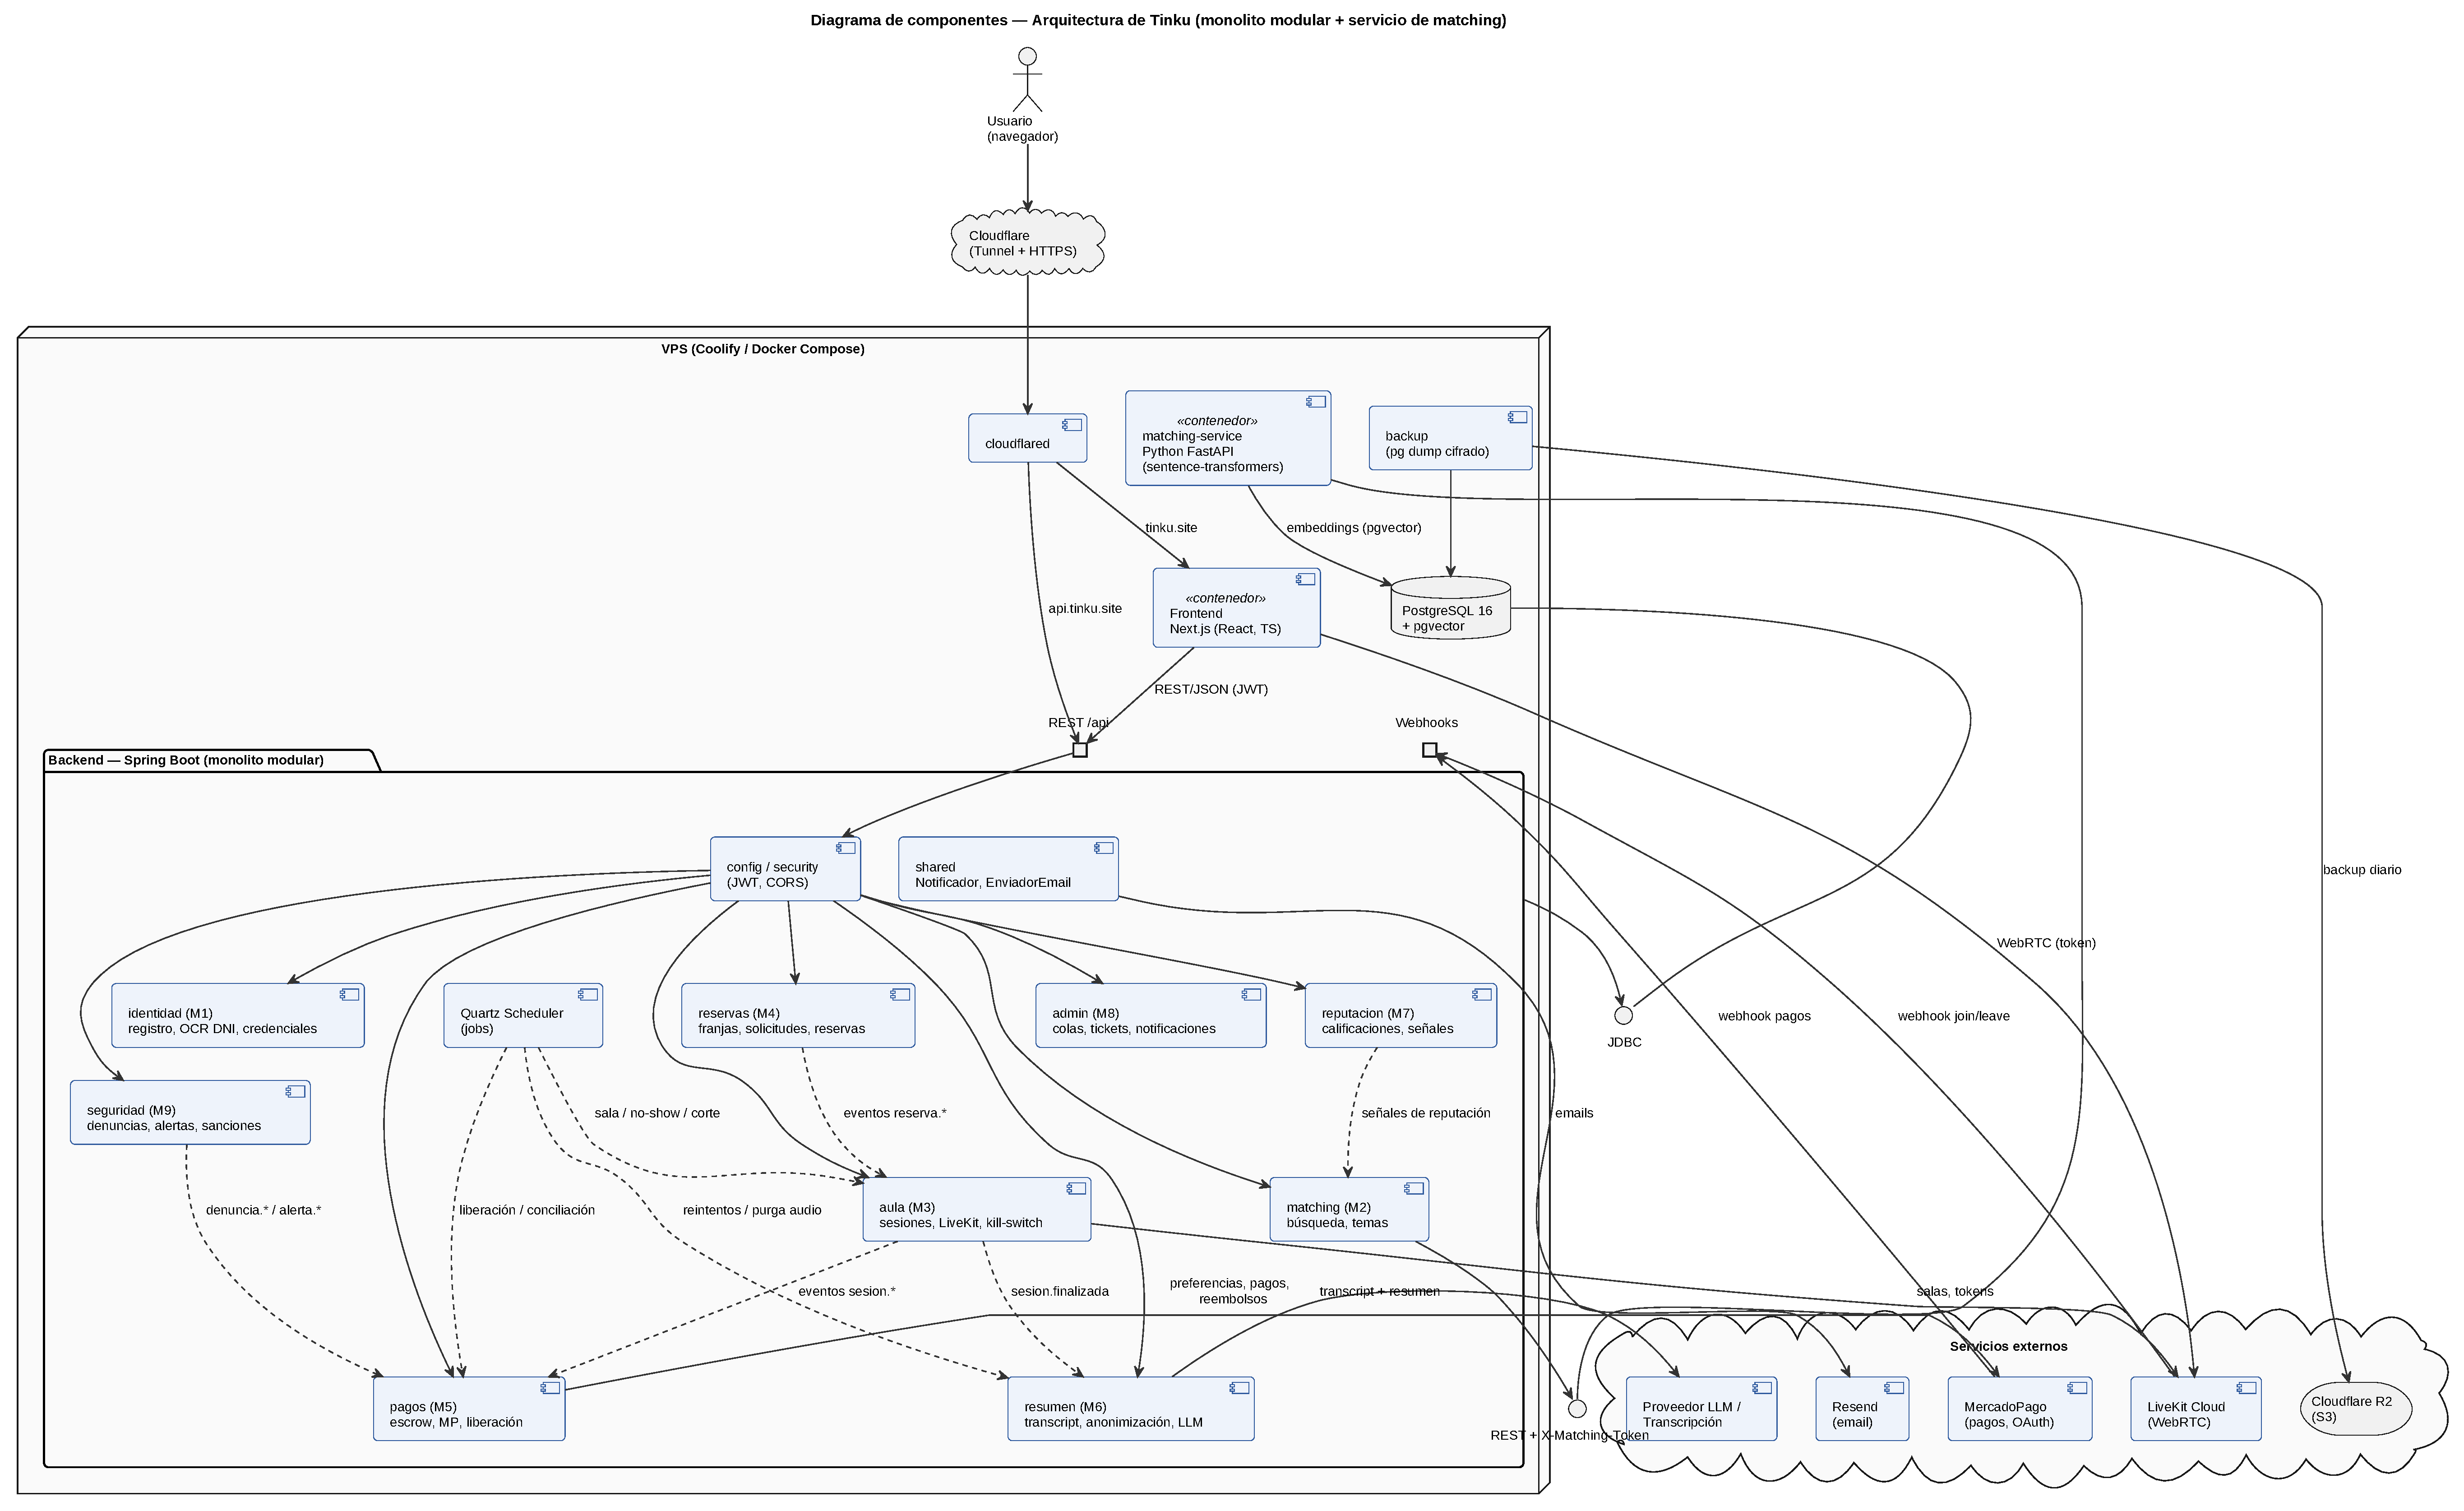
\includegraphics[width=\textwidth,height=0.8\textheight,keepaspectratio]{figuras/uml/09-componentes}
    \caption{Diagrama de componentes de Tinku}
    \label{fig:uml-componentes}
\end{figure}
